\documentclass{main}
\begin{document}
\section{Invisible Internet Project - I2P}
This is a project trying to implement \textbf{Garlic Routing} - A Routing protocol built over onion routing.
It is not used widely as of today because it needs slightly more technical knowledge to set up for
the first time for use. Also, the sites outside the network of invisible internet cannot be accessed
through the invisible internet. One may access outside internet through proxies (which do exist) but 
the proxies may be malicious and it may not be safe to do so. This also is a big problem hindering the
popularity of i2p.

\subsection{Structure of I2P: Components}
\begin{itemize}
	\item \textbf{Tunnel} \\
		Messages are sent from one node to another through tunnels. There are two tunnels, outbound tunnel
		and inbound tunnel. This is needed as per Garlic Routing protocol. The sender first builds an 
		outbound tunnel. It gets the details of Inbound tunnel from netDB. \\
		In a tunnel a gateway refers to first router and the last router is called endpoint.
		A user might have multiple such outbound and inbound tunnels. These tunnels
		used in I2P are \textbf{unidirectional} as opposed to bi-directional routes in Tor. \\
		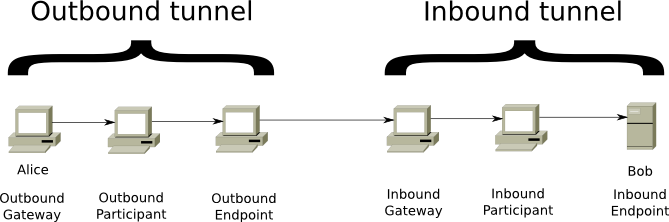
\includegraphics[width=0.95\textwidth]{Resources/images/i2p-tunnels.png}

		The sender adds routing instructions with the message, encrypts it and sends it through the tunnel.
		Just like Onion routing, this message is also encrypted using layered encryption. When the endpoint
		recieves the final message, it gets the routing instruction to the inbound gateway of reciever.
		The inbound gateway then sends this message to inbound endpoint through the tunnel. Except for this 
		difference, if we see tunnels as gateway to endpoint, both work in a similar way.

		Gateway accumulates some messages to be sent through the tunnel, adds path to reciever and
		converts them to \textbf{Garlic Message} so that they can be sent through tunnel.
		When the endpoint of tunnel finally decrypts the message, it separates the messages and forwards them 
		to the required hosts.
	\item \textbf{Network DataBase} \\
		Network Database stores the information about the routers present in the network. It also stores information
		about the tunnel gateways for inbound tunnels of users. In I2P, routers are identified by their public keys.
		This Network Database is a decentralized database. \\
		When a user wants to communicate with some other router in the Invisible Internet, he needs to lookup in the
		network database to find the details of inbound tunnel gateway for reciever. As it is a decentralized database,
		possibly, a router may not have access to complete database at any given time. As I2P is not widely used, it 
		is possible to find these details in a few tries but if the usage increases, it might become difficult to access
		this information.\\
		Network database stores two kinds of data: \textbf{Lease Sets} and \textbf{routerInfo}
\end{itemize}
\end{document}
